\subsubsection{SATs der Switches}
\paragraph{SATs}
\begin{figure}[!htb]
    \centering
    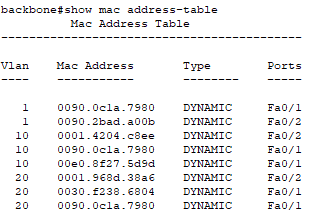
\includegraphics[width=.8\textwidth,keepaspectratio]{./img/SAT/BB.png}
    \caption{Backbone}
\end{figure}
\begin{figure}[!htb]
    \centering
    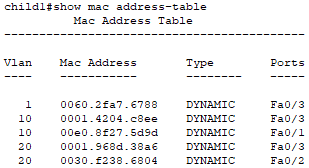
\includegraphics[width=.8\textwidth,keepaspectratio]{./img/SAT/S1.png}
    \caption{Access 1}
\end{figure}
\begin{figure}[!htb]
    \centering
    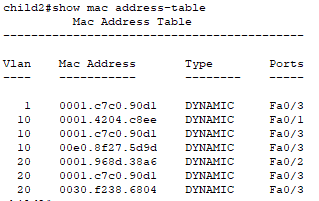
\includegraphics[width=.8\textwidth,keepaspectratio]{./img/SAT/S2.png}
    \caption{Access 2}
\end{figure}
\FloatBarrier

\subsubsection{Änderung der MAC Adresse}
\begin{figure}[!htb]
    \centering
    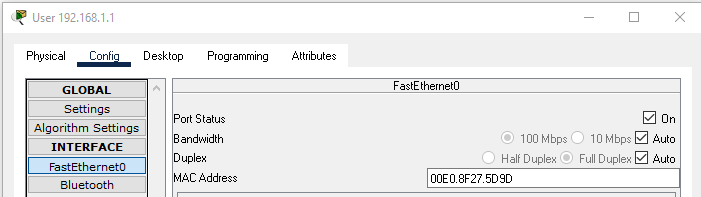
\includegraphics[width=.95\textwidth,keepaspectratio]{./img/SAT/MAC/PC1.png}
    \caption{Access 1}
\end{figure}
\begin{figure}[!htb]
    \centering
    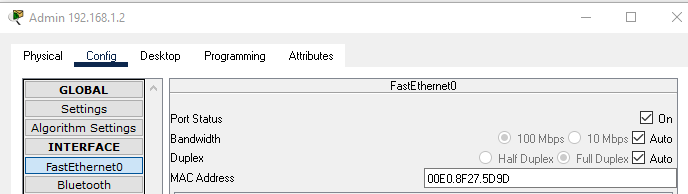
\includegraphics[width=.95\textwidth,keepaspectratio]{./img/SAT/MAC/PC2.png}
    \caption{Access 2}
\end{figure}
\FloatBarrier

\subsubsection{Frage 2}
\paragraph{Frage}
Welche MAC Adressen liegen an welchen Ports an, und zu welchen
Systemen gehören diese MAC Adresse, wie macht sich die doppelt vergebene
MAC-Adresse in der SAT bemerkbar, und wie sind die beiden Systeme mit
gleicher MAC-Adresse von anderen Systemen aus erreichbar und warum?
\paragraph{Antwort}

\begin{table}[!h]
    \centering
    \begin{tabular}{ |c|c|c| }
        \hline
        \thead{Gerät}     & \thead{Adresse} & \thead{Port}    \\
        \hline
        User 192.168.1.1  & 00E0.8F27.5D9D  & Switch 1, Fa0/1 \\
        \hline
        Admin 192.168.1.2 & 0030.F238.6804  & Switch 1, Fa0/2 \\
        \hline
        User 192.168.2.1  & 0001.4204.C8EE  & Switch 2, Fa0/1 \\
        \hline
        Admin 192.168.2.2 & 0001.968D.38A6  & Switch 2, Fa0/2 \\
        \hline
    \end{tabular}
\end{table}
\pagebreak
\paragraph{Resultate nach der Änderung}
Auf dem Switch 1, wo das Endsystem anhängt, wurde nur die Mac-Adresse auf dem jewiligen Port geändert.
Auf dem Backbone und dem Switch 2 wurde in der Tabelle die alte Adresse entfernt und die neue Adresse mit den gleichen Parametern hinzugefügt.

Das Systeme mit den gleichen Adressen sind wie zuvor von den zugeordneten Systemen erreichbar. Dies ist möglich, da die 2 Adressen auf 2 getrennten logischen Netzen liegen. Durch die Vlan Tags wissen die Switches wohin die Packets hin müssen.
\begin{figure}[!htb]
    \centering
    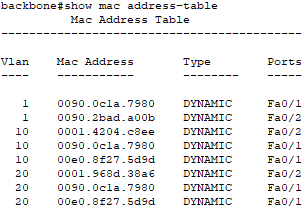
\includegraphics[width=.8\textwidth,keepaspectratio]{./img/SAT/Result/BB.png}
    \caption{Backbone}
\end{figure}
\begin{figure}[!htb]
    \centering
    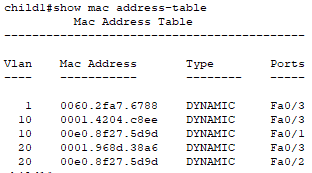
\includegraphics[width=.8\textwidth,keepaspectratio]{./img/SAT/Result/S1.png}
    \caption{Access 1}
\end{figure}
\begin{figure}[!htb]
    \centering
    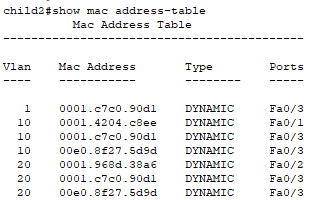
\includegraphics[width=.8\textwidth,keepaspectratio]{./img/SAT/Result/S2.png}
    \caption{Access 2}
\end{figure}
\FloatBarrier